% !TeX program = lualatex

\documentclass[smaller,xcolor=table,aspectratio=169]{beamer}

\usepackage{listings}
\usepackage[table]{xcolor}
\usepackage{array}

% Useful for writing out a space character
% See https://tex.stackexchange.com/a/50807
\newcommand\Vtextvisiblespace[1][.3em]{%
  \mbox{\kern.06em\vrule height.3ex}%
  \vbox{\hrule width#1}%
  \hbox{\vrule height.3ex}}



\mode<presentation>
{
	\usetheme{PrincetonJunction}
	\setbeamercovered{invisible}
}

\usetikzlibrary{arrows,arrows.meta,decorations.markings,fit,positioning,calc,shapes.geometric,shapes.symbols,shadows.blur,shadings,decorations.pathmorphing}

% For torn paper effect (see https://tex.stackexchange.com/questions/86150/torn-page-effect/86151#86151)
\pgfmathsetseed{1} % To have predictable results
% Define a background layer, in which the parchment shape is drawn
\pgfdeclarelayer{background}
\pgfsetlayers{background,main}
% This is the base for the fractal decoration. It takes a random point between the start and end, and
% raises it a random amount, thus transforming a segment into two, connected at that raised point
% This decoration can be applied again to each one of the resulting segments and so on, in a similar
% way of a Koch snowflake.
\pgfdeclaredecoration{irregular fractal line}{init}
{
  \state{init}[width=\pgfdecoratedinputsegmentremainingdistance]
  {
    \pgfpathlineto{\pgfpoint{random*\pgfdecoratedinputsegmentremainingdistance}{(random*\pgfdecorationsegmentamplitude-0.02)*\pgfdecoratedinputsegmentremainingdistance}}
    \pgfpathlineto{\pgfpoint{\pgfdecoratedinputsegmentremainingdistance}{0pt}}
  }
}

% Macro to draw the shape behind the text, when it fits completly in the
% page
\def\tornpaper#1{
\tikz{
  \node[inner sep=0] (A) {#1};  % Draw the text of the node
  \begin{pgfonlayer}{background}  % Draw the shape behind
  \fill[paper] % recursively decorate the bottom border
        decorate[irregular border]{decorate{decorate{decorate{decorate[ragged border]{
        (A.south east) -- (A.south west)
        %($(A.south east) - (0, random*5mm)$) -- ($(A.south west) - (0, random*5mm)$)
        }}}}}
        -- (A.north west) -- (A.north east) -- cycle;
  \end{pgfonlayer}}
}


\title[NLP Course 1]{Natural Language Processing}

\subtitle{Text, Numbers, and Computers}

% - Use the \inst{?} command only if the authors have different
%   affiliation.
\author{Phil Killewald}

% - Use the \inst command only if there are several affiliations.
% - Keep it simple, no one is interested in your street address.
% \institute[Universities of]
% {
% \inst{1}Department of Computer Science, Univ of S
% \and
% \inst{2}Department of Theoretical Philosophy, Univ of E
% }

% Should also contain the venue
\venue{Part of the Mathematica Advanced Analytics Training Series}
\location{Course 1 of N}
\date{Originally written in August of 2018}

% This is only inserted into the PDF information catalog. Can be left
% out.
\subject{Courses}



% Then you can add a logo as follows:
\pgfdeclareimage[height=5cm]{big-m}{logos/m-impact_blue_rays.pdf}
\titlegraphic{\pgfuseimage{big-m}}
\pgfdeclareimage[height=18pt]{mathematica-logo}{logos/m-impact_blue_rays.pdf}
\logo{\pgfuseimage{mathematica-logo}}

% Delete this if you do not want the table of contents to pop up at
% the beginning of each subsection:
\AtBeginSubsection[]
{
\begin{frame}<beamer>
\frametitle{Outline}
\tableofcontents[currentsection,currentsubsection]
\end{frame}
}

% If you wish to uncover everything in a step-wise fashion, uncomment
% the following command:
%\beamerdefaultoverlayspecification{<+->}

\begin{document}

% Useful for making pieces of a tikz appear with overlays
% See https://tex.stackexchange.com/a/55849
\tikzset{
	invisible/.style={opacity=0,text opacity=0},
	visible on/.style={alt={#1{}{invisible}}},
	alt/.code args={<#1>#2#3}{%
		\alt<#1>{\pgfkeysalso{#2}}{\pgfkeysalso{#3}} % \pgfkeysalso doesn't change the path
	},
	>=stealth,
	paper/.style={draw=black!10, blur shadow, fill=white, inner sep=0},
	irregular border/.style={decoration={irregular fractal line, amplitude=0.2},
		decorate,
	},
	ragged border/.style={ decoration={random steps, segment length=5mm, amplitude=1mm},
		decorate,
	}
}

{%
	\logo{\rule{0pt}{\beamerfootheight}}%
	\begin{frame}[noframenumbering]%
		\titlepage%
	\end{frame}%
}

%\begin{frame}
%\frametitle{Outline}
%\tableofcontents
% You might wish to add the option [pausesections]
%\end{frame}


\section{Introduction to Natural Language Processing}

\def\alicetext{{\rmfamily\small CHAPTER I. Down the Rabbit-Hole}\\[2ex]
Alice was beginning to get very tired of sitting by her sister on the
bank, and of having nothing to do\ldots}

% This is a nice color for the background, and provides a good way to highlight
% charts etc. with a white background.
\setbeamercolor{background canvas}{bg=mathematica light neutral}

\begin{frame}[plain]
	\begin{center}
		\begin{tikzpicture}[
		doc/.style={minimum width=2.10cm, minimum height=2.97cm, inner sep=.1 cm, align=left, node font=\tiny\ttfamily, text width=1.90cm, fill=white, draw=black},
		black box/.style={inner sep=.5cm, node font=\huge\bfseries, text=white, fill=mathematica grey, draw=black, thick},
		mathy/.style={inner sep=.5cm, text=black, fill=white, draw=black, thick, rounded corners=0.25cm, align=center},
		idea/.style={starburst, inner sep=0.25cm, text=white, draw=white, fill=mathematica red, ultra thick, node font=\Large\bfseries}
		]
			\begin{scope}[transparency group, visible on=<2->]
				\node[doc, blur shadow, rotate=rand*2] (doc3) {};
				\node[doc, rotate=rand*2] (doc2) at ($(doc3) + (-0.05cm,0.05cm)$) {};
				\node[doc, rotate=rand*2] (doc1) at ($(doc2) + (-0.05cm,0.05cm)$) {\alicetext};
			\end{scope}

			\node[black box, right=of doc2, visible on=<3->] (nlp) {NLP};
			\draw[->, thick, visible on=<3->] (doc2.north east) to [bend left=45] (nlp);

			\node[black box, cloud, visible on=<2>] (question) at (nlp) {?};

			\node[mathy, right=of nlp] (mat) {
			$\begin{bmatrix}
				x_{11} & x_{12} & \dots \\
				x_{21} & x_{22} & \\
				\vdots & & \ddots \\
			\end{bmatrix}$};
			\draw[->, thick, visible on=<3->] (nlp) to (mat);

			\node[mathy, right=of mat] (func) {$f(X) \sim y$};
			\draw[->,thick] (mat) to [bend left=45] (func);

			\node[idea, below=of func] (insight) {Insight!};
			\draw[->,thick] (func) to (insight);
			\draw[->,thick,dashed,visible on=<3->] (nlp) to [bend right=10] (insight);

			\node[anchor=north west, text width=.7\textwidth, align=left] (text) at ($(doc1.south west) + (0, -.8cm)$) {
			\begin{itemize}
				\item Statistical inference is Mathematica's bread \& butter.
				% \begin{itemize}
				% 	\item Map observations (matrix rows) of variables (matrix columns) to outcomes (vector) using linear models.
				% 	\item Variables and outcomes take numeric values.
				% \end{itemize}
				\item<2-> Surveys, interviews, social media, etc. produce copious amounts of human-generated free text.
				% \begin{itemize}
				% 	\item<2-> Free text does not fit into statistical inference algorithms.
				% 	\item<2-> We could pay for lots of people to code the text as numeric variables, but there must be a better way\ldots
				% \end{itemize}
				\item<3-> Enter {\bfseries Natural Language Processing: computer-based methods of converting human-generated text into meaningful quantitative data}.
			\end{itemize}
			};
		\end{tikzpicture}
	\end{center}
\end{frame}

\setbeamercolor{background canvas}{bg=white}

\newcommand{\deftext}[3]{{\huge\bfseries #1}\\[2em]{\color{mathematica grey}#2}\\[3em]#3}

\begin{frame}
	\frametitle{Definition}
	\framesubtitle{(for the purposes of this course)}
	\deftext{Natural Language Processing}{/ˈnætʃəɹəl/ /ˈlæŋɡwɪd͡ʒ/ /ˈpɹɑsəsɪŋ/}{``\textit{Computer-based methods} of converting \textit{human-generated text} into \textit{meaningful quantitiative data}.''}
\end{frame}

\begin{frame}[t]
	\frametitle{Relevant Published NLP Research}
	\tornpaper{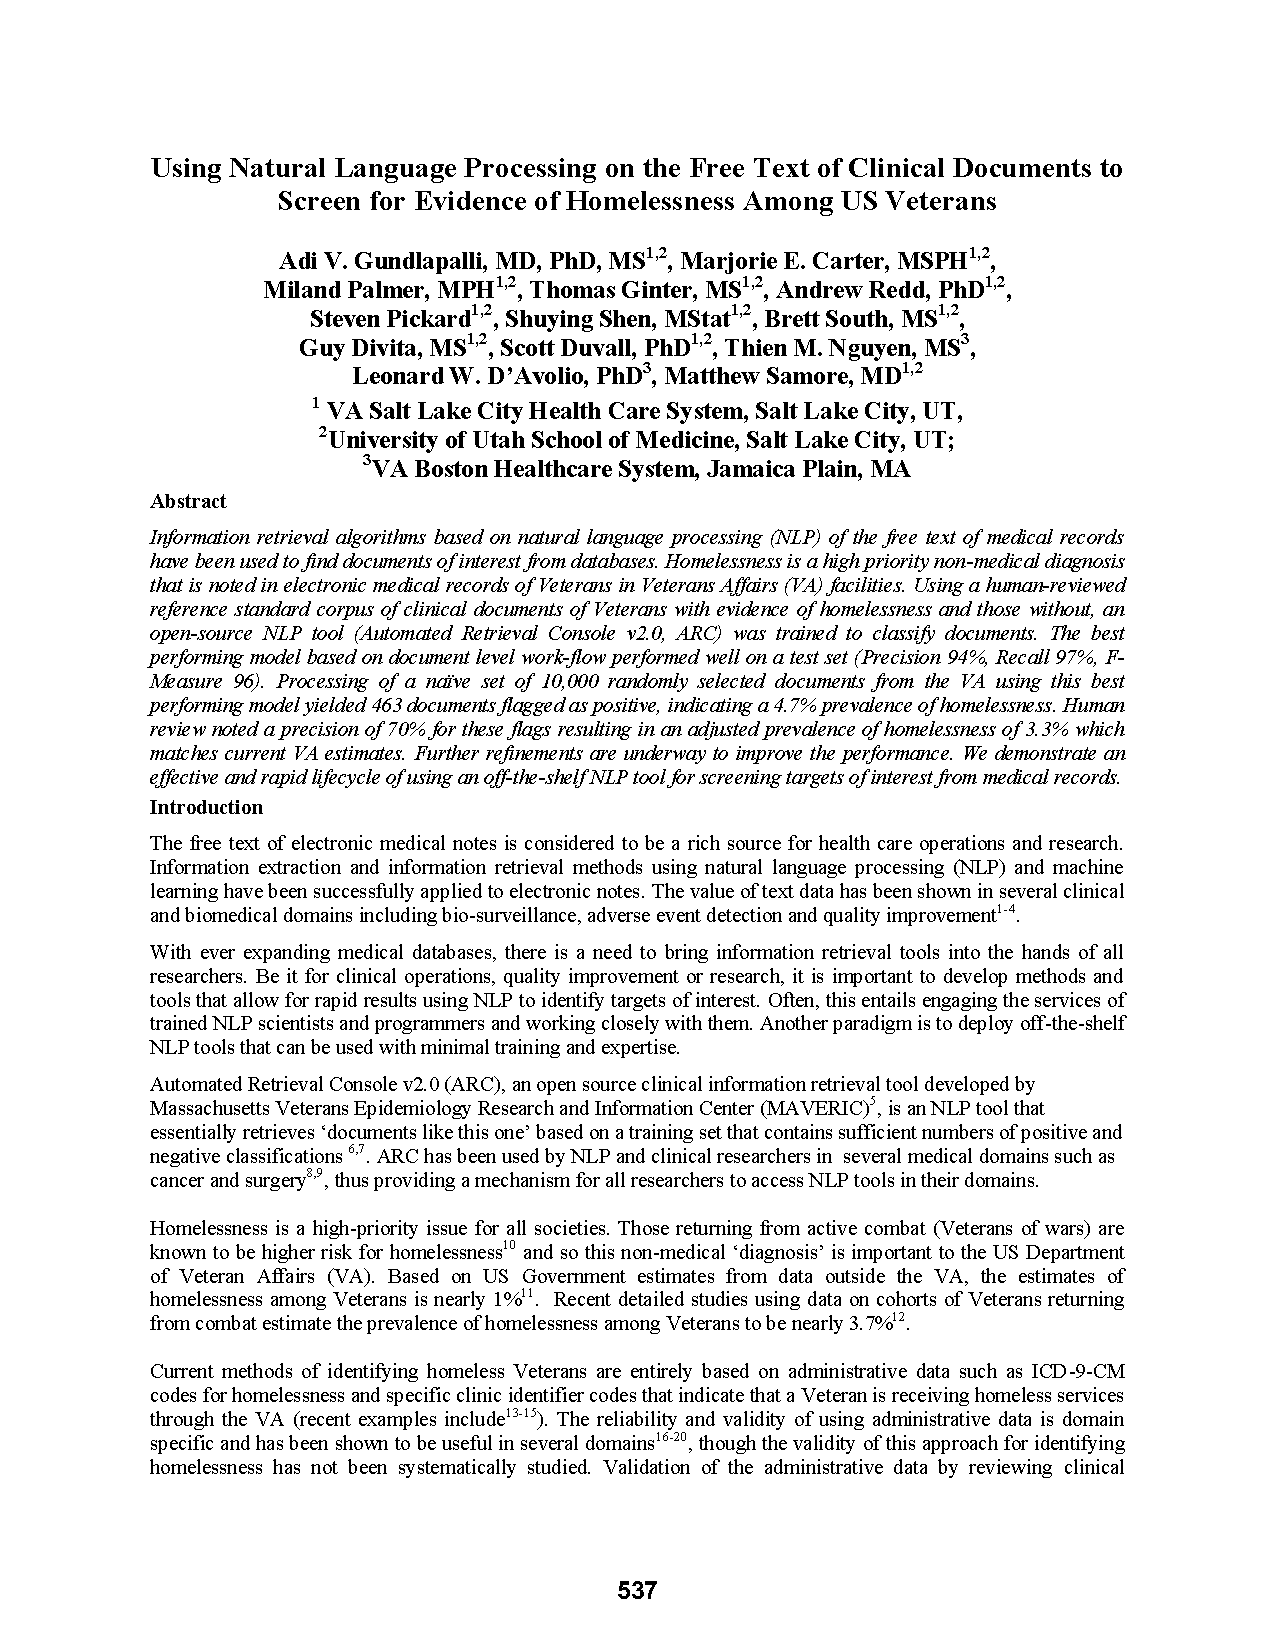
\includegraphics[page=1,width=0.3\textwidth,bb=0 7.5in 8.5in 11in,clip]{images/gundlapalli-amia-2013.pdf}}
	\tornpaper{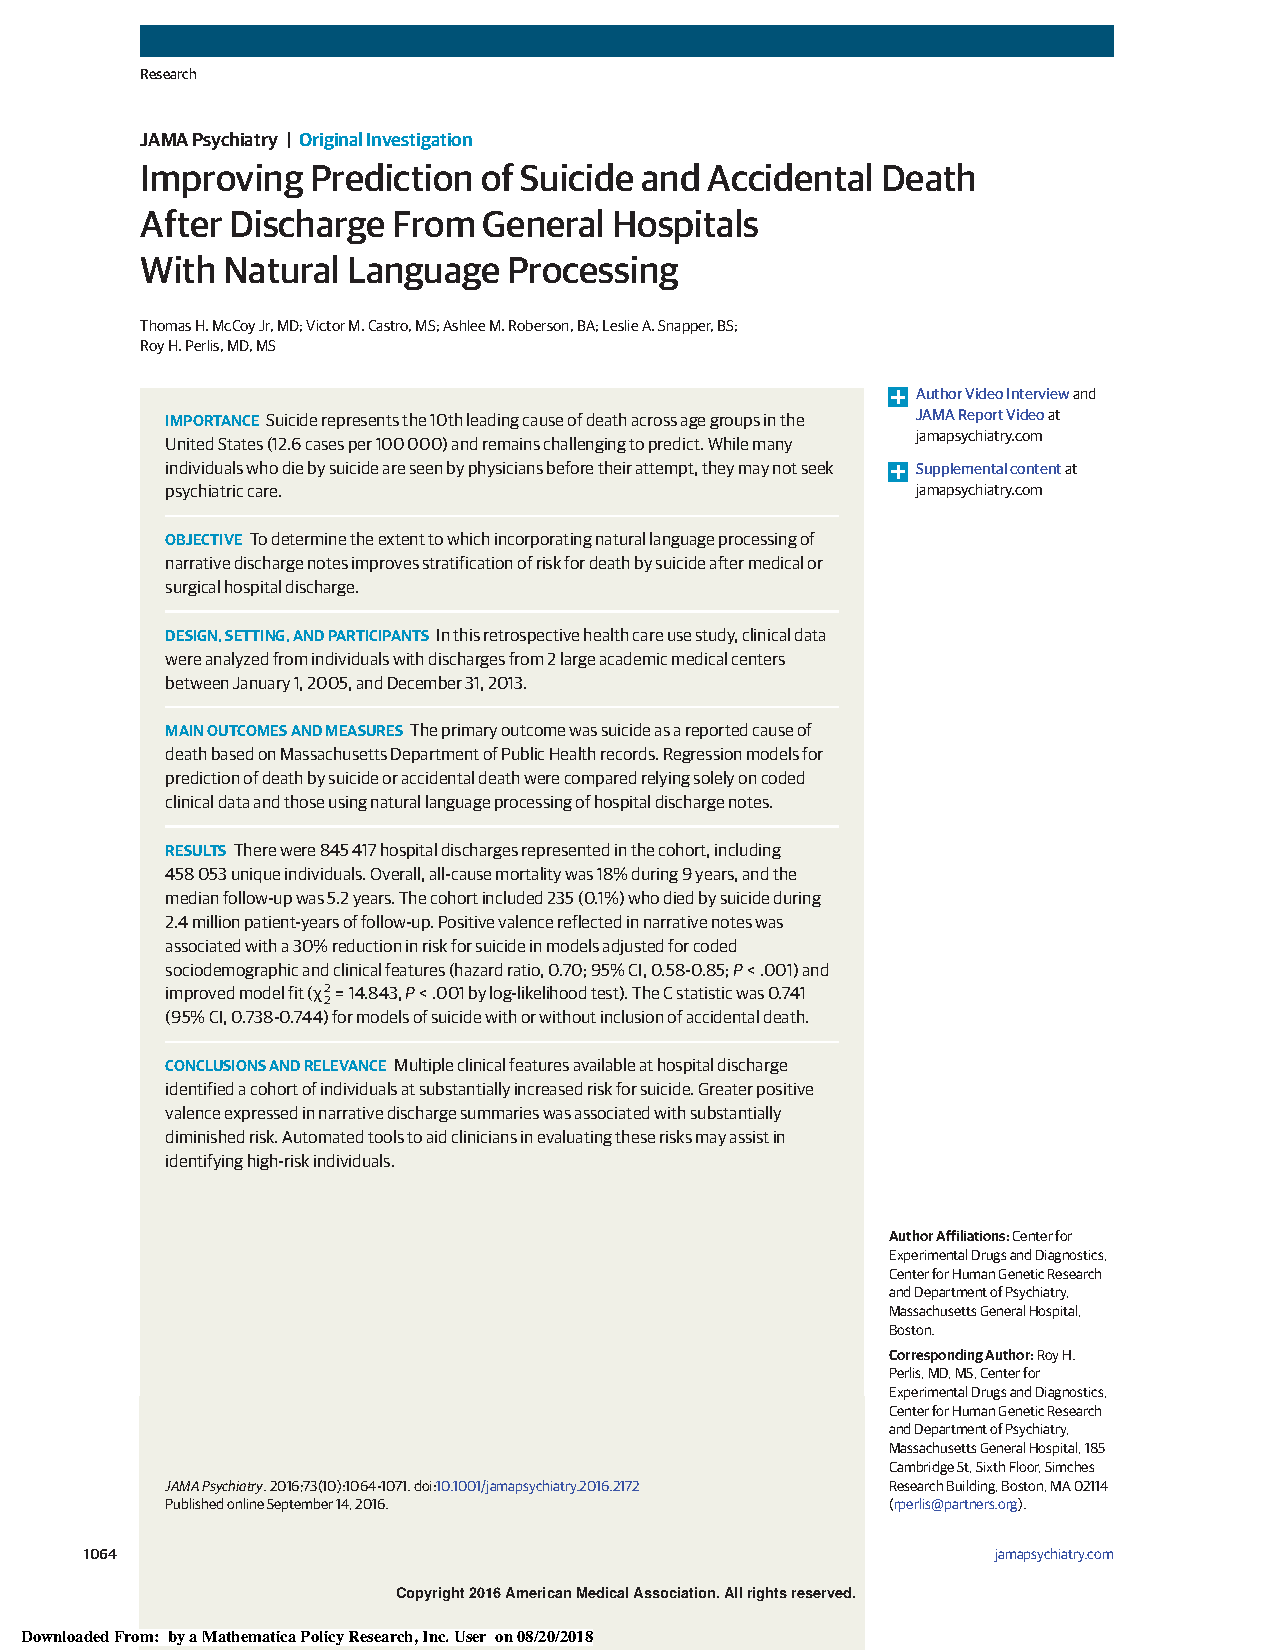
\includegraphics[page=1,width=0.3\textwidth,bb=0 7.5in 8.5in 11in,clip]{images/mccoy-jama-2016.pdf}}
	\tornpaper{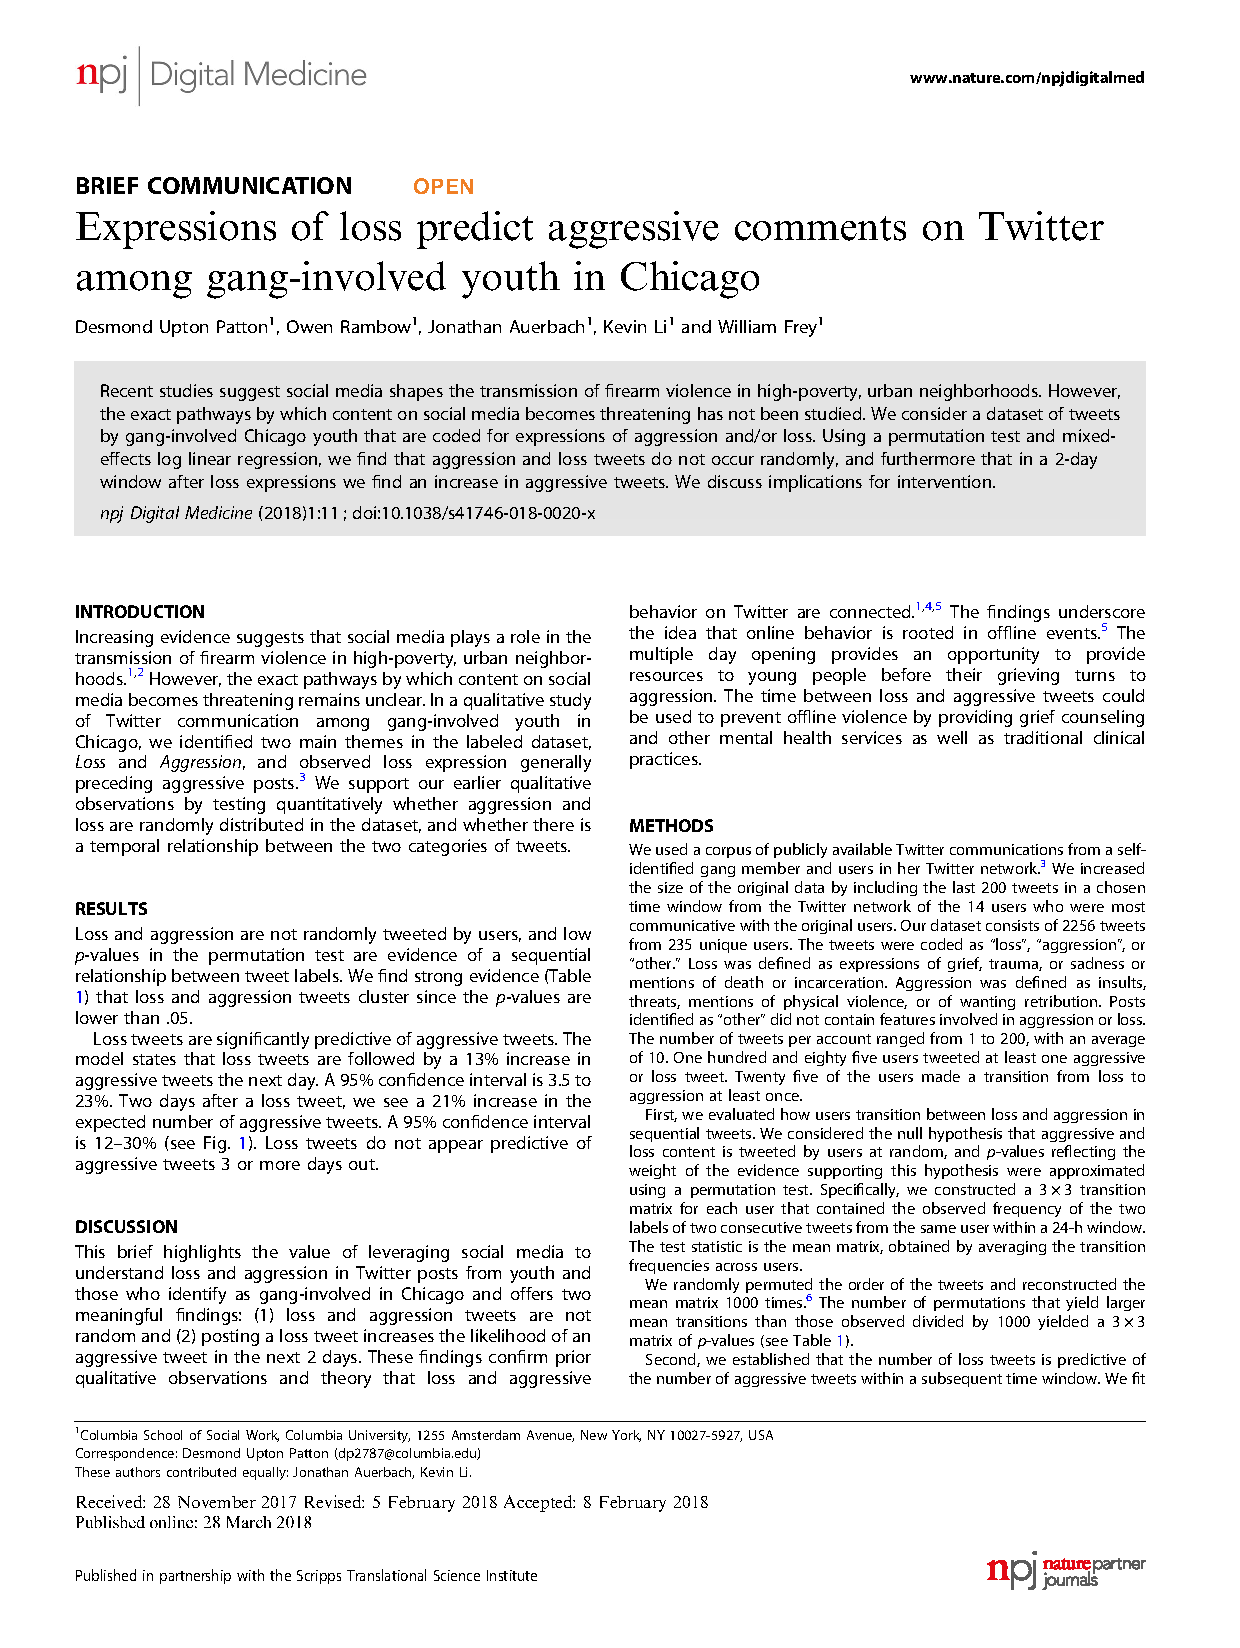
\includegraphics[page=1,width=0.3\textwidth,bb=0 7.5in 8.5in 11in,clip]{images/patton-npj-2018.pdf}}\\

	\begin{itemize}
		\item Gundlapalli, et al. (2013)--Identifying homelessness in US veterans by processing free-text fields in medical records
		\item McCoy, et al. (2016)--Stratifying suicide risk for patients discharged from medical or surgical facilities using narritive discharge notes
		\item Patton, et al. (2018)--Correlating expressions of loss and expressions of aggression in gang-involved youth Twitter data
	\end{itemize}

\end{frame}


\begin{frame}
	\frametitle{Course Timeline}
	\begin{center}
		\begin{tikzpicture}[
			]
			\draw[->, mathematica grey, thick] (0,0) -- (0,-6cm);
			\foreach \y/\label [count=\i] in {-.5/Introduction and Tokenization,-1.5/Preprocessing,-2.5/``Classical'' NLP,-3.5/Frequency Methods,-4.5/Embeddings,-5.5/State-of-the-Art NLP}
				{
					\coordinate (c\i) at (0,\y cm);
					\draw[mathematica grey] (-2pt,\y cm) -- (2pt,\y cm);
					\node[right=0.5cm of c\i] {Course \i: \label};
				}
			\draw[->|, very thick, mathematica red] (0, 0) -- (c1);
			\node[right=0.5 of c1, text=mathematica red] {Course 1: Introduction and Tokenization};
		\end{tikzpicture}
	\end{center}
	% \begin{enumerate}
	% 	\item Course Introduction
	% 	\item Computer Representation of Text \& Canned Libraries
	% 	\item Preparing Text
	% 	\item Traditional NLP
	% 	\item Quantification of Text
	% 	\item Modern Quantification of Text
	% 	\item State-of-the-Art Quantification of Text
	% \end{enumerate}
\end{frame}

% \begin{frame}[fragile]
% 	\frametitle{Example Documents}
% 	\begin{center}
% 		\begin{tikzpicture}[font=\scriptsize,
% 				container/.style={rectangle, anchor=north, inner sep=3mm, rounded corners=3mm,
% 					draw=mathematica blue, text=mathematica blue, thick},
% 				communicant/.style={rectangle, anchor=center,
% 					rounded corners=1mm, color=white},
% 				communique/.style={shape=ellipse, anchor=center,
% 					color=mathematica dark blue, draw=mathematica dark blue, align=center},
% 				top label/.style={rectangle, anchor=base west,
% 					text=mathematica blue, fill=white, font=\small}]
% 				\node[matrix, column sep=3mm, row sep=3mm] (m1) {
% 					\node[communicant, fill=mathematica dark blue]
% 					(doctors)
% 					{Doctor}; &
% 					\node[communique]
% 					(notes)
% 					{doctor's\\notes}; &
% 					\node[communicant, fill=mathematica brown]
% 					(medics)
% 					{Medical Staff}; \\
%
% 					\node[communicant, fill=mathematica dark blue, visible on=<2->]
% 					(clerk)
% 					{Clerk}; &
% 					\node[communique, visible on=<2->]
% 					(minutes)
% 					{minutes}; &
% 					\node[communicant, fill=mathematica brown, visible on=<2->]
% 					(public)
% 					{Public}; \\
%
% 					\node[communicant, fill=mathematica dark blue, visible on=<3->]
% 					(reporter)
% 					{Reporter}; &
% 					\node[communique, visible on=<3->]
% 					(scrawl)
% 					{shorthand\\scrawl}; & \\
% 				};
%
% 				\draw[->] (doctors) to (notes) to (medics);
% 				\draw[->, visible on=<2->] (clerk) to (minutes) to (public);
% 				\draw[-, visible on=<3->] (reporter) to [out=15, in=165] (scrawl);
% 				\draw[->, visible on=<3->] (scrawl) to [out=195, in=-15] (reporter);
%
% 				\node[container, fit={(m1)}]
% 				(container1)
% 				{};
% 				\node[top label]
% 				at ($(container1.north west) + (3mm,0)$)
% 				{Professional Notes};
%
% 				\node[matrix, column sep=3mm, row sep=3mm, right=of m1, visible on=<4->] (m2) {
% 					\node[communicant, fill=mathematica dark blue]
% 					(legislators)
% 					{Legislators}; &
% 					\node[communique]
% 					(laws)
% 					{laws}; &
% 					\node[communicant, fill=mathematica brown]
% 					(populace)
% 					{Populace}; \\
%
% 					\node[communicant, fill=mathematica dark blue]
% 					(president)
% 					{President}; &
% 					\node[communique]
% 					(executive order)
% 					{executive\\orders}; &
% 					\node[communicant, fill=mathematica brown]
% 					(government)
% 					{Executive Branch}; \\
%
% 					\node[communicant, fill=mathematica dark blue]
% 					(servant)
% 					{Civil Servants}; &
% 					\node[communique]
% 					(fr)
% 					{Federal\\Register}; &
% 					\node[communicant, fill=mathematica brown]
% 					(wonks)
% 					{Policy Wonks}; \\
% 				};
%
% 				\draw[->, visible on=<4->] (legislators) to (laws) to (populace);
% 				\draw[->, visible on=<4->] (president) to (executive order) to (government);
% 				\draw[->, visible on=<4->] (servant) to (fr) to (wonks);
%
% 				\node[container, fit={(m2)}, visible on=<4->]
% 				(container2)
% 				{};
% 				\node[top label, visible on=<4->]
% 				at ($(container2.north west) + (3mm,0)$)
% 				{Laws and Policies};
%
% 				\end{tikzpicture}
% 				\\
% 				\begin{tikzpicture}[visible on=<5->, font=\scriptsize,
% 						container/.style={rectangle, anchor=north, inner sep=3mm, rounded corners=3mm,
% 							draw=mathematica blue, text=mathematica blue, thick},
% 						communique/.style={shape=ellipse, anchor=center,
% 							color=mathematica dark blue, draw=mathematica dark blue, align=center},
% 						top label/.style={rectangle, anchor=base west,
% 							text=mathematica blue, fill=white, font=\small}]
%
% 						\node[matrix, column sep=12mm] (m3) {
% 							\node[communique] (transcripts) {interview\\transcriptions}; &
% 							\node[communique] (academic) {academic\\papers}; &
% 							\node[communique] (wikipedia) {Wikipedia\\articles}; &
% 							\node[communique] (random) {random\\websites}; \\
% 						};
%
% 						\foreach \n in {transcripts,academic,wikipedia,random} {
% 							\draw[dotted] ($(\n.west) + (-3mm,0)$)
% 							to ($(\n.west)$);
% 							\draw[->,dotted] ($(\n.east)$)
% 							to ($(\n.east) + (3mm,0)$);
% 						}
%
% 						\node[container, fit={(m3)}]
% 						(container3)
% 						{};
% 						\node[top label]
% 						at ($(container3.north west) + (3mm,0)$)
% 						{Other Common Documents};
%
% 						\end{tikzpicture}
% 						\end{center}
% 						\end{frame}







						\section{Computer Representations of Text}

						\begin{frame}
							\frametitle{Bytes}
							Computers understand bytes.\\\pause{}
							Byte: an 8-digit binary number\\\pause{}
							Bytes can take values from 0 to 255.\\\pause{}
							Everything a computer does is based around bytes:\\\pause{}
							\begin{itemize}
								\item Integer math
								\item Booleans
								\item Floating point operations
								\item File reading/writing
								\item Literally everything
							\end{itemize}
							But people understand glyphs
						\end{frame}

						\begin{frame}
							\frametitle{ASCII}
							Ancient computers communicated everything using bytes.\\
							\includegraphics[width=.5\textwidth]{images/eniac.jpg}\pause{}\\
							This was annoying.
						\end{frame}

						\newcommand{\CNT}{\cellcolor{mathematica green!25}}
						\newcommand{\ALP}{\cellcolor{mathematica orange!25}}
						\newcommand{\PUN}{\cellcolor{mathematica purple!25}}
						\begin{frame}[plain]
							(American) computer scientists developed a way for computers to represent text for input and output purposes.\\
							ASCII: American Standard Code for Information Interchange\\
							Standard that encodes numbers 0 through 127 (0x00 through 0x7F) as Latin glyphs.\\
							\begin{table}
								\tiny\ttfamily
								\begin{tabular}{r|c|c|c|c|c|c|c|c|c|c|c|c|c|c|c|c}
									    & \_0                     & \_1      & \_2      & \_3      & \_4      & \_5      & \_6      & \_7      & \_8      & \_9     & \_A      & \_B      & \_C                 & \_D     & \_E                   & \_F      \\ \hline
									0\_ & \CNT nul                & \CNT soh & \CNT stx & \CNT etx & \CNT eot & \CNT enq & \CNT ack & \CNT bel & \CNT bs  & \CNT ht & \CNT lf  & \CNT vt  & \CNT ff             & \CNT cr & \CNT so               & \CNT si  \\
									1\_ & \CNT dle                & \CNT dc1 & \CNT dc2 & \CNT dc3 & \CNT dc4 & \CNT nak & \CNT syn & \CNT etb & \CNT can & \CNT em & \CNT sub & \CNT esc & \CNT fs             & \CNT gs & \CNT rs               & \CNT us  \\
									2\_ & \PUN \Vtextvisiblespace & \PUN !   & \PUN "   & \PUN \#  & \PUN \$  & \PUN \%  & \PUN \&  & \PUN '   & \PUN (   & \PUN )  & \PUN *   & \PUN +   & \PUN ,              & \PUN -  & \PUN .                & \PUN /   \\
									3\_ & \ALP 0                  & \ALP 1   & \ALP 2   & \ALP 3   & \ALP 4   & \ALP 5   & \ALP 6   & \ALP 7   & \ALP 8   & \ALP 9  & \PUN :   & \PUN ;   & \PUN <              & \PUN =  & \PUN >                & \PUN ?   \\
									4\_ & \PUN @                  & \ALP A   & \ALP B   & \ALP C   & \ALP D   & \ALP E   & \ALP F   & \ALP G   & \ALP H   & \ALP I  & \ALP J   & \ALP K   & \ALP L              & \ALP M  & \ALP N                & \ALP O   \\
									5\_ & \ALP P                  & \ALP Q   & \ALP R   & \ALP S   & \ALP T   & \ALP U   & \ALP V   & \ALP W   & \ALP X   & \ALP Y  & \ALP Z   & \PUN [   & \PUN \textbackslash & \PUN ]  & \PUN \textasciicircum & \PUN \_  \\
									6\_ & \PUN `                  & \ALP a   & \ALP b   & \ALP c   & \ALP d   & \ALP e   & \ALP f   & \ALP g   & \ALP h   & \ALP i  & \ALP j   & \ALP k   & \ALP l              & \ALP m  & \ALP n                & \ALP o   \\
									7\_ & \ALP p                  & \ALP q   & \ALP r   & \ALP s   & \ALP t   & \ALP u   & \ALP v   & \ALP w   & \ALP x   & \ALP y  & \ALP z   & \PUN \{  & \PUN |              & \PUN \} & \PUN \textasciitilde  & \CNT del \\
								\end{tabular}
							\end{table}
						\end{frame}

						\newcommand{\UND}{\cellcolor{black}\color{white}}
						\begin{frame}[plain]
							Problems with ASCII:\\\pause{}
							Other languages use more glyphs than those in American English:\\\pause{}
							\begin{itemize}
								\item £
								\item ¿
								\item á
								\item «»
							\end{itemize}\pause{}
							Temporary solution: use that 8th bit!\\
							\begin{table}
								\footnotesize
								\begin{tabular}{r|c|c|c|c|c|c|c|c|c|c|c|c|c|c|c|c}
									    & \_0                    & \_1                    & \_2                    & \_3                    & \_4                    & \_5                    & \_6                    & \_7                    & \_8                   & \_9                    & \_A                   & \_B                    & \_C                   & \_D      & \_E                   & \_F                   \\ \hline
									8\_ & \UND {\visible<5->€} & \UND                   & \UND {\visible<5->‚} & \UND {\visible<5->ƒ}  & \UND {\visible<5->„} & \UND {\visible<5->…} & \UND {\visible<5->†} & \UND {\visible<5->‡} & \UND {\visible<5->ˆ} & \UND {\visible<5->‰} & \UND {\visible<5->Š} & \UND {\visible<5->‹} & \UND {\visible<5->Œ} & \UND     & \UND {\visible<5->Ž} & \UND                  \\
									9\_ & \UND                   & \UND {\visible<5->‘} & \UND {\visible<5->’} & \UND {\visible<5->“} & \UND {\visible<5->”} & \UND {\visible<5->•} & \UND {\visible<5->–} & \UND {\visible<5->—} & \UND {\visible<5->˜} & \UND {\visible<5->™} & \UND {\visible<5->š} & \UND {\visible<5->›} & \UND {\visible<5->œ} & \UND     & \UND {\visible<5->ž} & \UND {\visible<5->Ÿ} \\
									A\_ & \PUN nbsp              & \PUN ¡                & \PUN ¢                & \PUN £                & \PUN ¤                & \PUN ¥                & \PUN ¦                & \PUN §                & \PUN ¨               & \PUN ©                & \PUN ª               & \PUN «                & \PUN ¬               & \PUN shy & \PUN ®               & \PUN ¯               \\
									B\_ & \PUN °                & \PUN ±                & \ALP ²                & \ALP ³                & \PUN ´                & \ALP µ                & \PUN ¶                & \PUN ·                & \PUN ¸               & \ALP ¹                & \PUN º               & \PUN »                & \ALP ¼               & \ALP ½  & \ALP ¾               & \PUN ¿               \\
									C\_ & \ALP À                & \ALP Á                & \ALP Â                & \ALP Ã                & \ALP Ä                & \ALP Å                & \ALP Æ                & \ALP Ç                & \ALP È               & \ALP É                & \ALP Ê               & \ALP Ë                & \ALP Ì               & \ALP Í  & \ALP Î               & \ALP Ï               \\
									D\_ & \ALP Ð                & \ALP Ñ                & \ALP Ò                & \ALP Ó                & \ALP Ô                & \ALP Õ                & \ALP Ö                & \PUN ×                & \ALP Ø               & \ALP Ù                & \ALP Ú               & \ALP Û                & \ALP Ü               & \ALP Ý  & \ALP Þ               & \ALP ß               \\
									E\_ & \ALP à                & \ALP á                & \ALP â                & \ALP ã                & \ALP ä                & \ALP å                & \ALP æ                & \ALP ç                & \ALP è               & \ALP é                & \ALP ê               & \ALP ë                & \ALP ì               & \ALP í  & \ALP î               & \ALP ï               \\
									F\_ & \ALP ð                & \ALP ñ                & \ALP ò                & \ALP ó                & \ALP ô                & \ALP õ                & \ALP ö                & \PUN ÷                & \ALP ø               & \ALP ù                & \ALP ú               & \ALP û                & \ALP ü               & \ALP ý  & \ALP þ               & \ALP ÿ               \\
								\end{tabular}
							\end{table}
							{\visible<5->Windows:  Looks like you forgot some curley quote marks, so I fixed it for you. (Windows-1252)}
						\end{frame}

						\newfontface\hebfont{NotoSansHebrew}[Scale=MatchLowercase]
						\newfontface\chkfont{NotoSansCherokee}[Scale=MatchLowercase]
						% \newfontface\chnfont{NotoSansCJKsc}[Scale=MatchLowercase]
						\newcommand{\hebtxt}[1]% Hebrew text inside LTR
						{\bgroup\textdir TRT\hebfont #1\egroup}

						\begin{frame}
							\frametitle{Problems}
							Turns out there are languages out there other than those that use forms of the Latin alphabet.
							\begin{itemize}
								\item<1-> hello world
								\item<2-> Здравствуй, мир (ru)
								\item<3-> {\chkfont ᎣᏏᏲ ᎡᎶᎯ} (ck)
								% \item<4-> {\chnfont 你好世界} (cn)
							\end{itemize}
						\end{frame}

						\begin{frame}
							\frametitle{Unicode}
							Solution:  Variable-width encoding (specifically, UTF-8)
							Advantages:
							\begin{itemize}
								\item Large number of symbols ($17$ {\em planes} of $2^{16}$ {\em code points})
								\item Backwards-compatable with ASCII (7-bit) and some extended ASCII (8-bit) symbols
							\end{itemize}
							Disadvantages:
							\begin{itemize}
								\item Lengths of strings are hard
								      \begin{itemize}
								      	\item Number of bytes != number of code points
								      	\item Number of code points != number of glyphs
								      \end{itemize}
								\item Microsoft is difficult
								      \begin{itemize}
								      	\item Curly quotes, elipses, dashes, bullets, etc. in {\em continuation code} space of UTF-8
								      \end{itemize}
							\end{itemize}
						\end{frame}

						\newfontface\emojifont{NotoEmoji-Regular}
						\begin{frame}
							\frametitle{Examples}
							\begin{table}
								\small
								\begin{tabular}{|c|c|c|c|c|c|c|c|c|}
									\hline
									48 & 69 & 2c & 20                 & 77 & 6f & 72 & 6c & 64 \\ \hline
									H  & i  & ,  & \Vtextvisiblespace & w  & o  & r  & l  & d  \\ \hline
								\end{tabular}
							\end{table}

							% \begin{table}
							% 	\small
							% 	\begin{tabular}{|c c c|c c c|c c c|c c c|}
							% 		\hline
							% 		e4 & bd & a0 & e5 & a5 & bd & e4 & b8 & 96 & e7 & 95 & 8c \\ \hline
							% 		\multicolumn{3}{|c|}{\chnfont 你} & \multicolumn{3}{c|}{\chnfont 好} & \multicolumn{3}{c|}{\chnfont 世} & \multicolumn{3}{c|}{\chnfont 界} \\ \hline
							% 	\end{tabular}
							% \end{table}

							\begin{table}
								\small
								\begin{tabular}{|c|c|c|c|c c c c|c c c c|}
									\hline
									48 & 69 & 2c & 20 & f0 & 9f & 87 & ba & f0 & 9f & 87 & b8 \\ \hline
									H & i & , & \Vtextvisiblespace & \multicolumn{4}{c|}{\emojifont 🇺} & \multicolumn{4}{c|}{\emojifont 🇸} \\ \hline
									H & i & , & \Vtextvisiblespace & \multicolumn{8}{c|}{\emojifont 🇺🇸} \\ \hline
								\end{tabular}
							\end{table}

							\begin{table}
								\small
								\begin{tabular}{|c|c|c c c|c|c|c|c|c|c|c|c c c|c|c|}
									\hline
									69 & 6e & ef & ac & 81 & 6e & 69 & 74 & 65 & 20 & 77 & 61 & ef & ac & 84 & 65 & 73 \\ \hline
									i & n & \multicolumn{3}{c|}{fi} & n & i & t & e & \Vtextvisiblespace & w & a & \multicolumn{3}{c|}{ffl} & e & s \\ \hline
									i & n & \multicolumn{3}{c|}{\begin{tabular}{c c} f & i\\ \end{tabular}} & n & i & t & e & \Vtextvisiblespace & w & a & f & f & l & e & s \\ \hline
								\end{tabular}
							\end{table}

						\end{frame}

						\begin{frame}
							\frametitle{Getting It Wrong}
							\begin{enumerate}
								\item Using the wrong encoding can make text undecypherable.
								\item Encoding information is out-of-band--you must be told what encoding to use.
								\item Nobody will have any idea what you are talking about.
							\end{enumerate}

							\begin{table}
								\small
								\begin{tabular}{|c|c|c|c|c|c|c|c|c|c|c|c|c|}
									\hline
									48 & 69 & 2c & 20 & f0 & 9f & 87 & ba & f0 & 9f & 87 & b8 & 21 \\ \hline
									H & i & , & \Vtextvisiblespace & \multicolumn{8}{c|}{\emojifont 🇺🇸} \\ \hline
									H & i & , & \Vtextvisiblespace & ð & Ÿ & ‡ & ° & ð & Ÿ & ‡ & ¸ \\ \hline
								\end{tabular}
							\end{table}
						\end{frame}

						\lstset{language=Python}
						\lstset{
							morekeywords={with,as},
							morekeywords=[2]{>>>}
						}
						\lstdefinestyle{mystyle}{
							basicstyle=\footnotesize\color{black}\ttfamily,
							backgroundcolor=\color{mathematica light neutral},
							showspaces=false,
							showtabs=false,
							breaklines=true,
							showstringspaces=false,
							breakatwhitespace=true,
							% Color settings
							keywordstyle=\color{mathematica brown}\bfseries, % core keywords
							keywordstyle={[2]\color{mathematica dark purple}\bfseries}, % built-ins
							keywordstyle={[3]\color{mathematica neutral}\bfseries}, % built-ins
							stringstyle=\color{mathematica dark green},
							commentstyle=\color{mathematica dark neutral}\itshape,
							upquote=true
						}

						\begin{frame}[fragile]
							\frametitle{Guessing (Intelligently)}
							chardet
							\begin{lstlisting}[style=mystyle]
>>> import urllib.request
>>> import chardet
>>> with urllib.request.urlopen('http://google.co.jp') as req:
>>>     rawdata = req.read()
>>>     for x in rawdata:
>>>         pass
>>>     chardet.detect(rawdata)
{'encoding': 'Windows-1252', 'confidence': 0.73, 'language': ''}
							\end{lstlisting}

						\end{frame}

						\section*{Summary}

						\begin{frame}
							\frametitle{Summary}
							\begin{itemize}
								\item NLP means a lot of things
								      \begin{itemize}
								      	\item For us at this point in time, we will focus on {\itshape quantification of written human communication}.
								      \end{itemize}
								\item As a rule, human communication is not meant for quantitative analysis.
								      \begin{itemize}
								      	\item We have to come up with ways of converting language into numbers carefully without sacraficing too much of the original meaning.
								      \end{itemize}
								\item Computers only understand numbers.
								      \begin{itemize}
								      	\item Computers represent text for input/output purposes using encodings.
								      	\item Encodings are one way of turning text into numbers.
								      	\item The universe of standard encodings is a mess, and you cannot control what encodings other people use.
								      \end{itemize}
							\end{itemize}
							\begin{alertblock}{Takeaway}
								Always use UTF-8 whenever you possibly can!
							\end{alertblock}
						\end{frame}

						\section*{Homework}

						\begin{frame}
							\frametitle{Homework}
							Encoding, Decoding, and Counting Glyphs
						\end{frame}

\end{document}
